\section[Theorie]{Theorie \textnormal{\cite{faraday}}}
\label{sec:theorie}

\subsection{Bandstruktur}

\begin{figure}
    \centering
    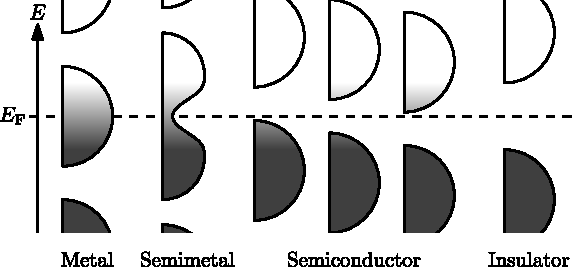
\includegraphics[width=0.8\textwidth]{content/grafik/bandstructure.pdf}
    \caption{Bandstrukturen verschiedener Materialklassen im Vergleich. \cite{wiki_band}}
    \label{fig:baender}
\end{figure}

\begin{figure}
    \centering
    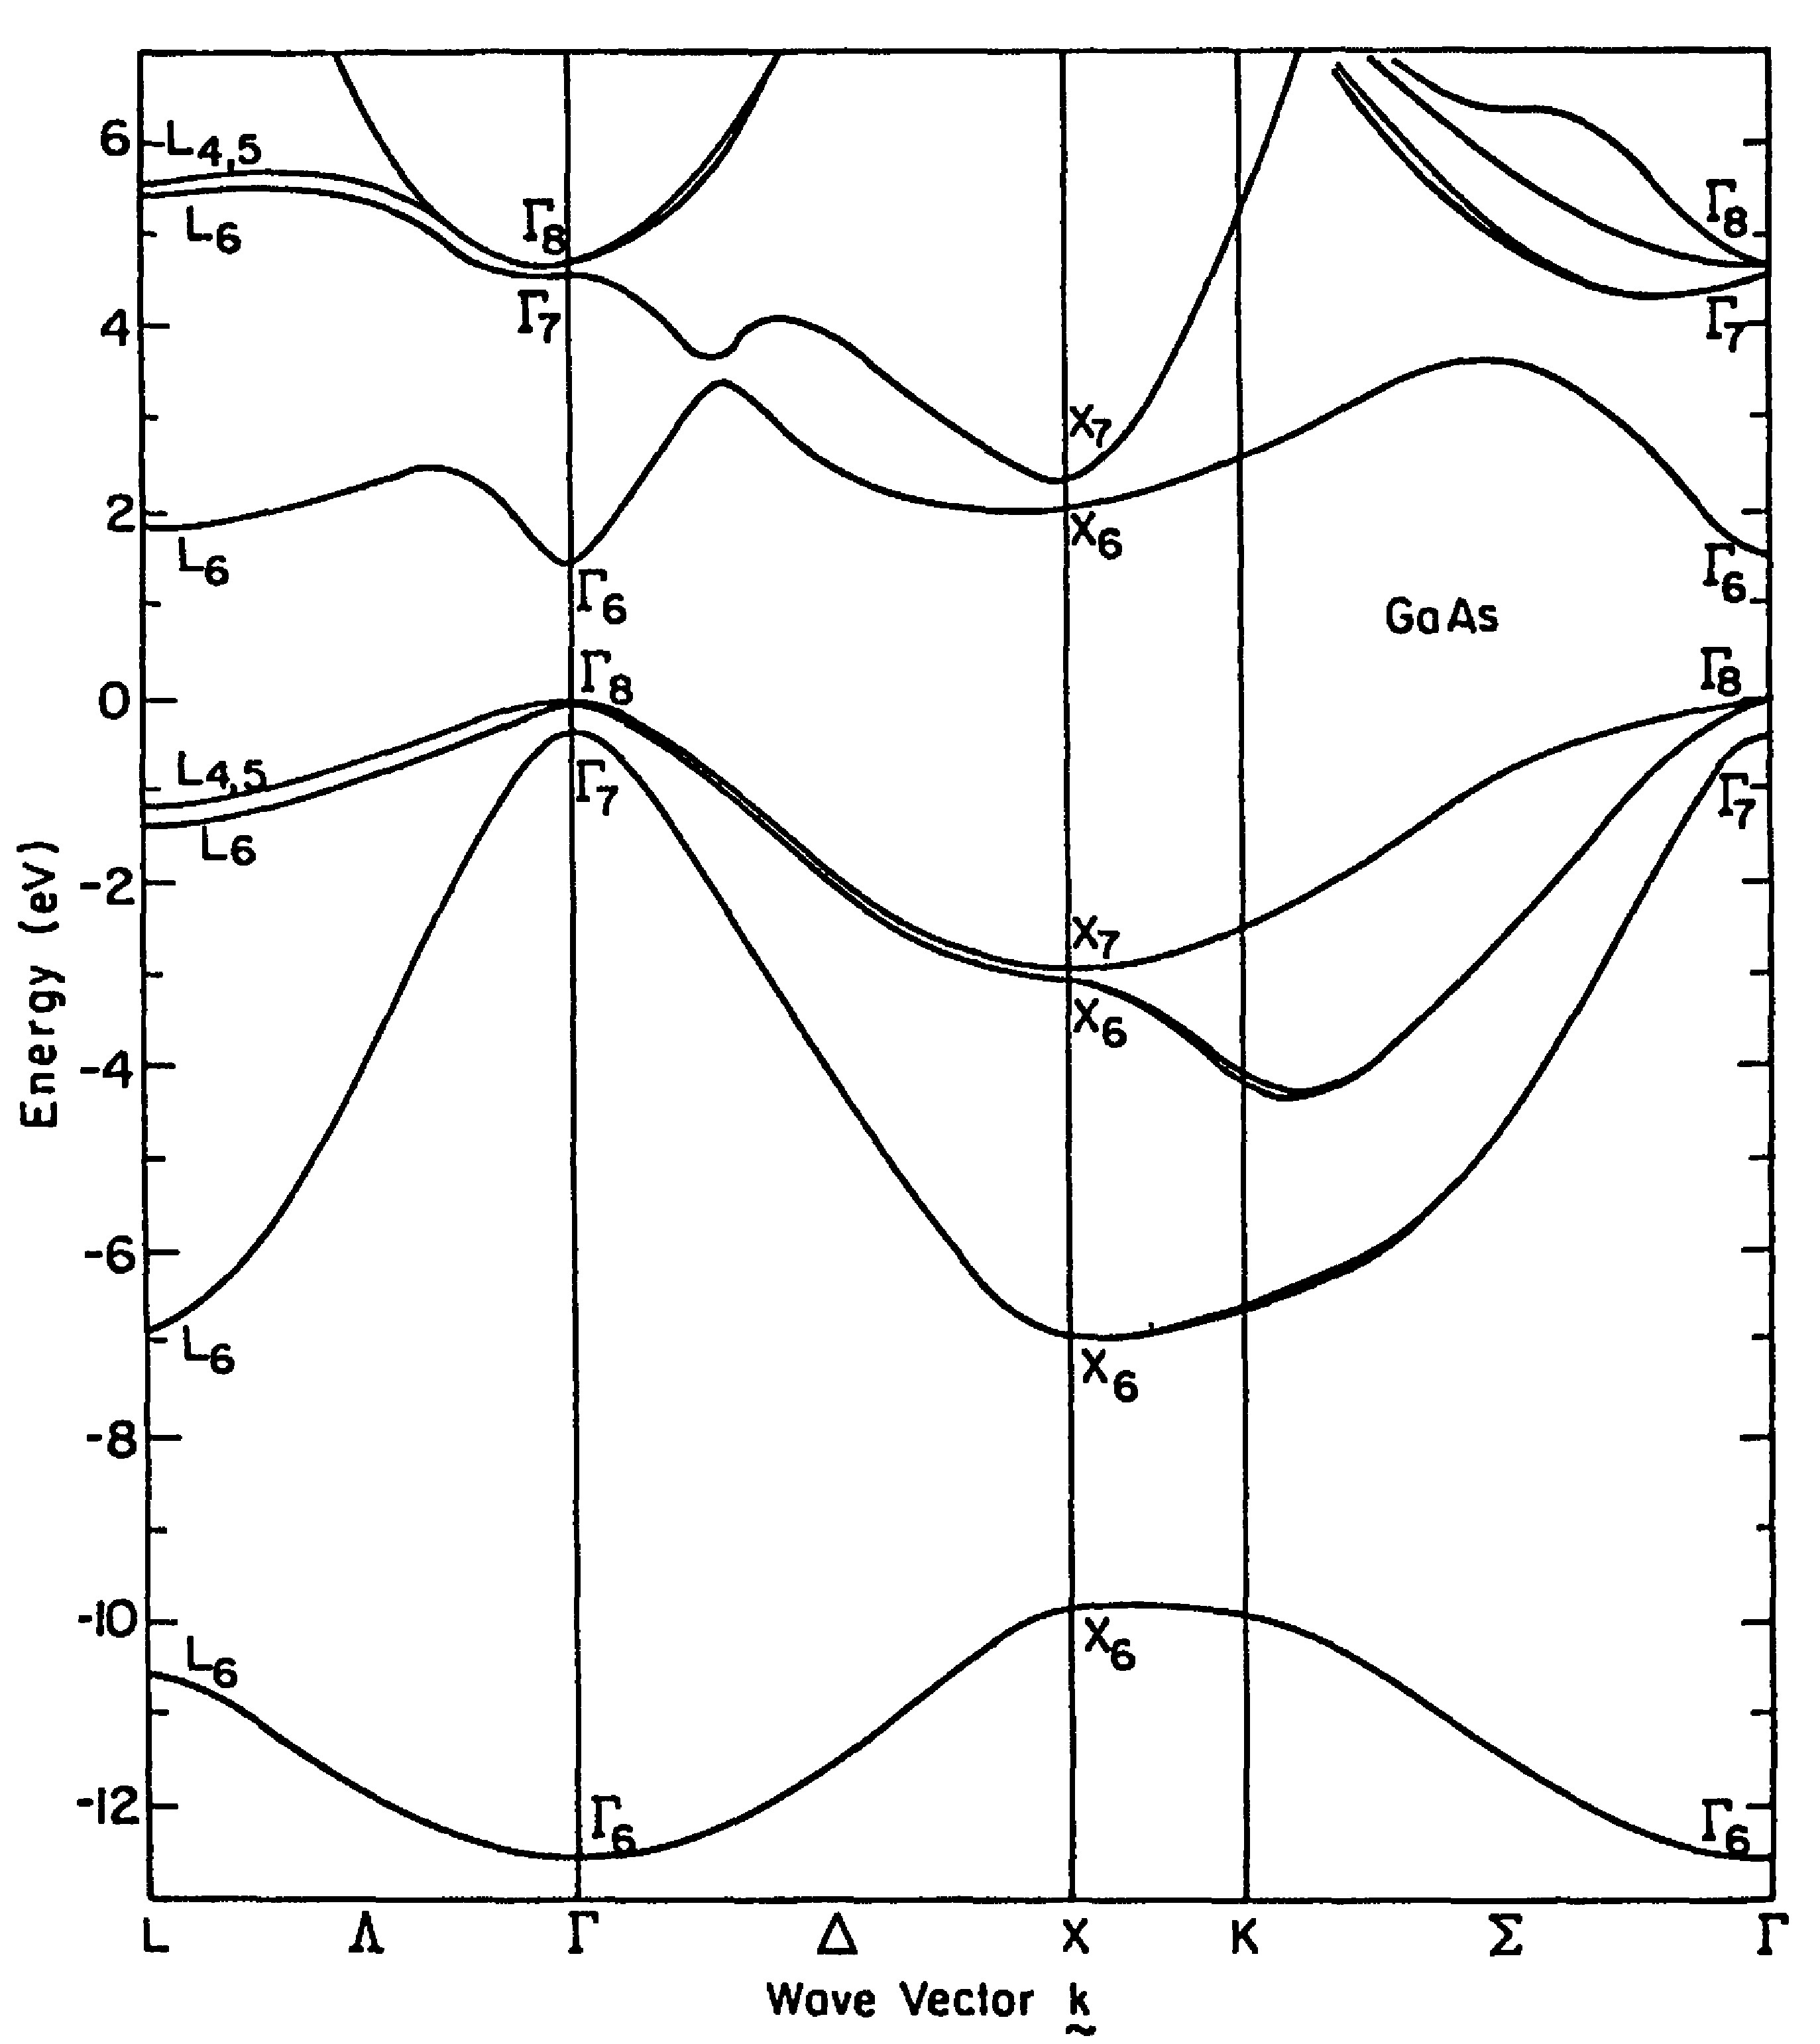
\includegraphics[width=0.6\textwidth]{content/grafik/bandstruktur.jpg}
    \caption{Berechnete Bandstruktur von GaAs um die Bandlücke. \cite{coh_jam_el}}
    \label{fig:band}
    \hfill
\end{figure}

\subsection{Dotierung}

\subsection{Faraday-Effekt}

\begin{figure}
    \centering
    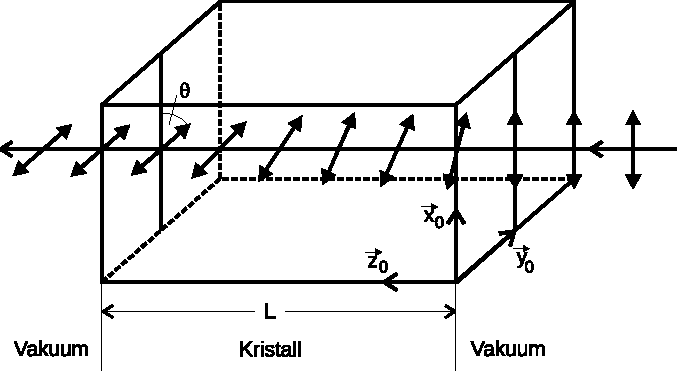
\includegraphics[width=0.7\textwidth]{content/grafik/drehung.pdf}
    \caption{Drehung der Polarisationsebene einer Lichtwelle beim Durchgang durch einen Kristall. \cite{faraday}}
    \label{fig:drehung}
    \hfill
\end{figure}
